\chapter{Introducción}

La astrosismología es el estudio de las oscilaciones estelares mediante el análisis de los cambios que estas provocan en la luz de las estrellas \citep{ChristensenDalsgaard2019}. Dichos cambios se manifiestan como pequeñas variaciones en el brillo (fotometría) o como desplazamientos en las líneas espectrales debido al efecto Doppler (espectroscopía), y permiten obtener información acerca de la estructura interior, composición química e historia evolutiva de las estrellas.

Estas oscilaciones corresponden a modos propios de vibración atrapados en el interior de la estrella. El análisis de estos modos permite determinar con precisión los gradientes de densidad, la rotación interna del núcleo y la extensión de las zonas de mezcla convectiva, entre otros, proporcionando una visión de la estructura interna que la fotometría clásica no puede dilucidar \citep{ChristensenDalsgaard2019}.

En presente trabajo tiene como objetivo establecer, en el marco de la propuesta de misión HAYDN de la ESA \citep{haydn_mission_proposal_2026}, una distinción de estrellas con diferentes historias evolutivas mediante la astrosismología. En concreto, se estudiarán las denominadas \textit{Blue Stragglers} para comprobar si la astrosismología puede diferenciarlas de estrellas con historias evolutivas distintas que se encuentren en la misma posición aparente en el diagrama HR.

\section{\textit{Blue Stragglers}}

Los cúmulos estelares resultan ser de gran importancia a la hora de probar modelos teóricos de evolución estelar, puesto que permiten comparar sus predicciones con las observaciones. Esto se debe a que se asume que las estrellas de un mismo cúmulo se formaron alrededor del mismo momento y con una composición química muy similar (provienen de la misma nube de gas y polvo). Al asumir esto como verdadero, se puede estudiar en detalle cómo la masa inicial de una estrella determina su evolución a lo largo del tiempo sin la interferencia de otros parámetros desconocidos \citep{TASC8KASC15AbstractBooklet}.

Esta homogeneidad permite modelar la población de un cúmulo mediante el uso de isócronas: curvas teóricas en el diagrama HR que representan las posiciones de estrellas de la misma edad y composición química, pero con diferentes masas iniciales. A medida que el cúmulo envejece, las estrellas más masivas agotan el hidrógeno en su núcleo y abandonan la secuencia principal. El punto preciso del diagrama donde se produce esta transición se conoce como el ``\textit{turn-off point}'', y permite estimar la antigüedad de un cúmulo en concreto \citep{wang2024bluestragglerstars}.

\begin{figure}[H]
  \centering
  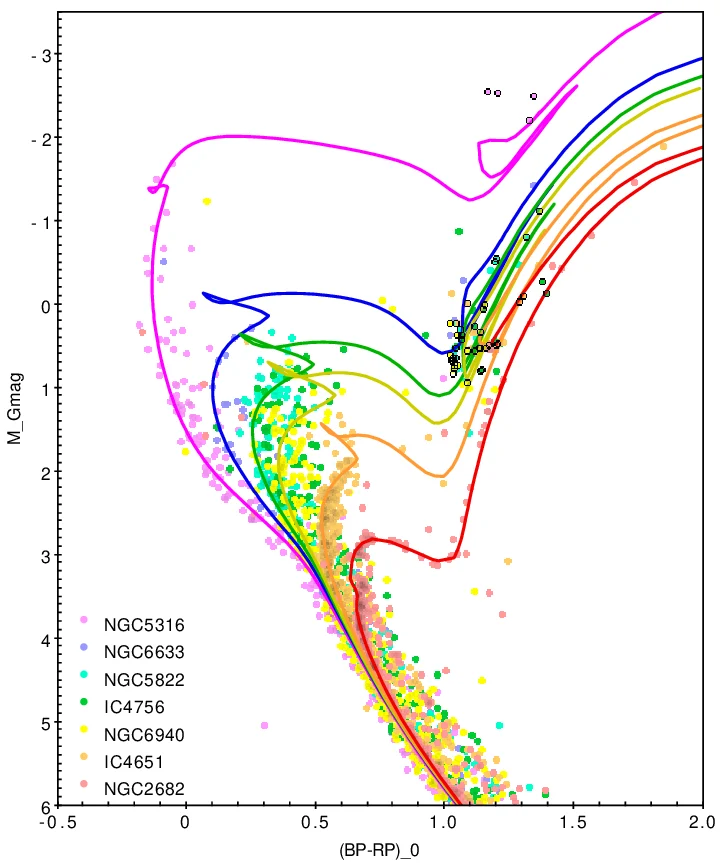
\includegraphics[width=0.8\textwidth]{Imagenes/HR_isoch.png}
  \caption{Diagrama HR para distintos cúmulos estelares con las isócronas de mejor ajuste superpuestas. Puede apreciarse el ``\textit{turn-off point}'' en diferentes posiciones dependiendo de la edad del cúmulo. Cuanto más a la derecha se encuentra este punto, más antiguo es el cúmulo. Imagen tomada de \citet{santrich_2022}.}
  \label{fig:hr_diagram}
\end{figure}

No obstante, al elaborar este tipo de diagramas, a menudo se observan una serie de anomalías que escapan a la explicación de los modelos estelares evolutivos simples. Un ejemplo de ello son las \textit{Blue Stragglers}, estrellas más calientes y luminosas que el resto de estrellas de un mismo cúmulo, y que, de alguna manera, parecen haber ``rejuvenecido'' (ya que se encuentran arriba y a la izquierda del \textit{turn-off point} de su cúmulo) \citep{wang2024bluestragglerstars}. Un ejemplo de este tipo de estrellas se puede apreciar en la Figura \ref{fig:hr_diagram_bss}.

\begin{figure}[H]
  \centering
  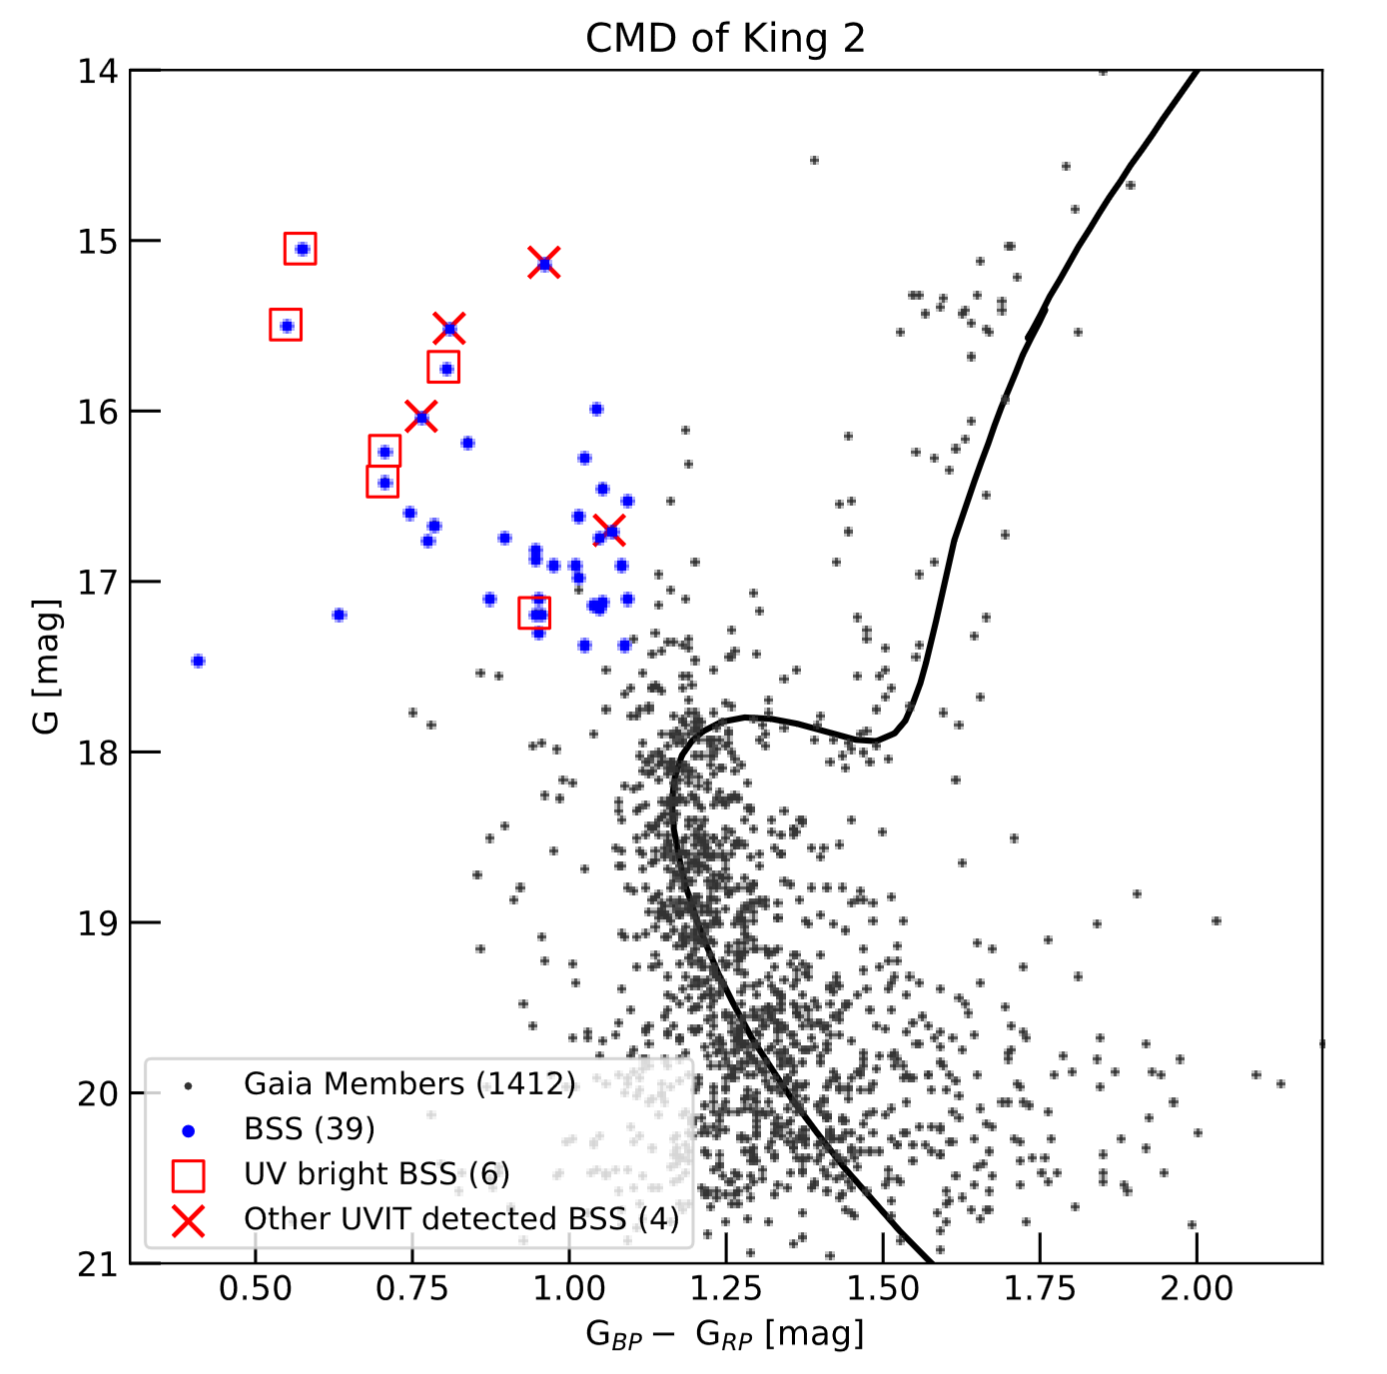
\includegraphics[width=0.65\textwidth]{Imagenes/HR_BSS.png}
  \caption{Diagrama HR de los miembros del cúmulo King 2. Las estrellas en azul conforman el grupo de \textit{Blue Stragglers} del cúmulo. La isócrona de mejor ajuste del cúmulo tiene los parámetros $\log(\text{edad}) = 9.7$, $\mathrm{[M/H]} = -0.4$, $\text{DM} = 13.8$ y $E(B-V) =0.45$. Figura tomada de \citet{Jadhav_2021}.}
  \label{fig:hr_diagram_bss}
\end{figure}

Frecuentemente, este tipo de estrellas se ubican en una zona del diagrama HR correspondiente a tres tipos de estrellas pulsantes: $\delta$ Scuti, $\gamma$ Doradus, y SX Phoenicis \citep{Kurtz2022, 10.3389/fspas.2022.952296}. Las $\delta$ Scuti oscilan en la zona correspondiente a modos p y g de bajo orden (alrededor del fundamental radial), las $\gamma$ Doradus oscilan en la zona correspondiente a modos g de alto orden (bajas frecuencias) y las SX Phoenicis, principalmente, en la zona correspondiente al fundamental radial y primer sobretono ($n_{\mathrm{pg}} = 0, 1$) \citep{Handler_2009,10.3389/fspas.2022.952296}. En el Capítulo 2 se profundizará acerca de estos modos de oscilación. Una imagen de la distribución de tipos de estrellas pulsantes en el diagrama HR se puede apreciar en la Figura \ref{fig:hr_diagram_pulsating_stars}.

\begin{figure}[t]
  \centering
  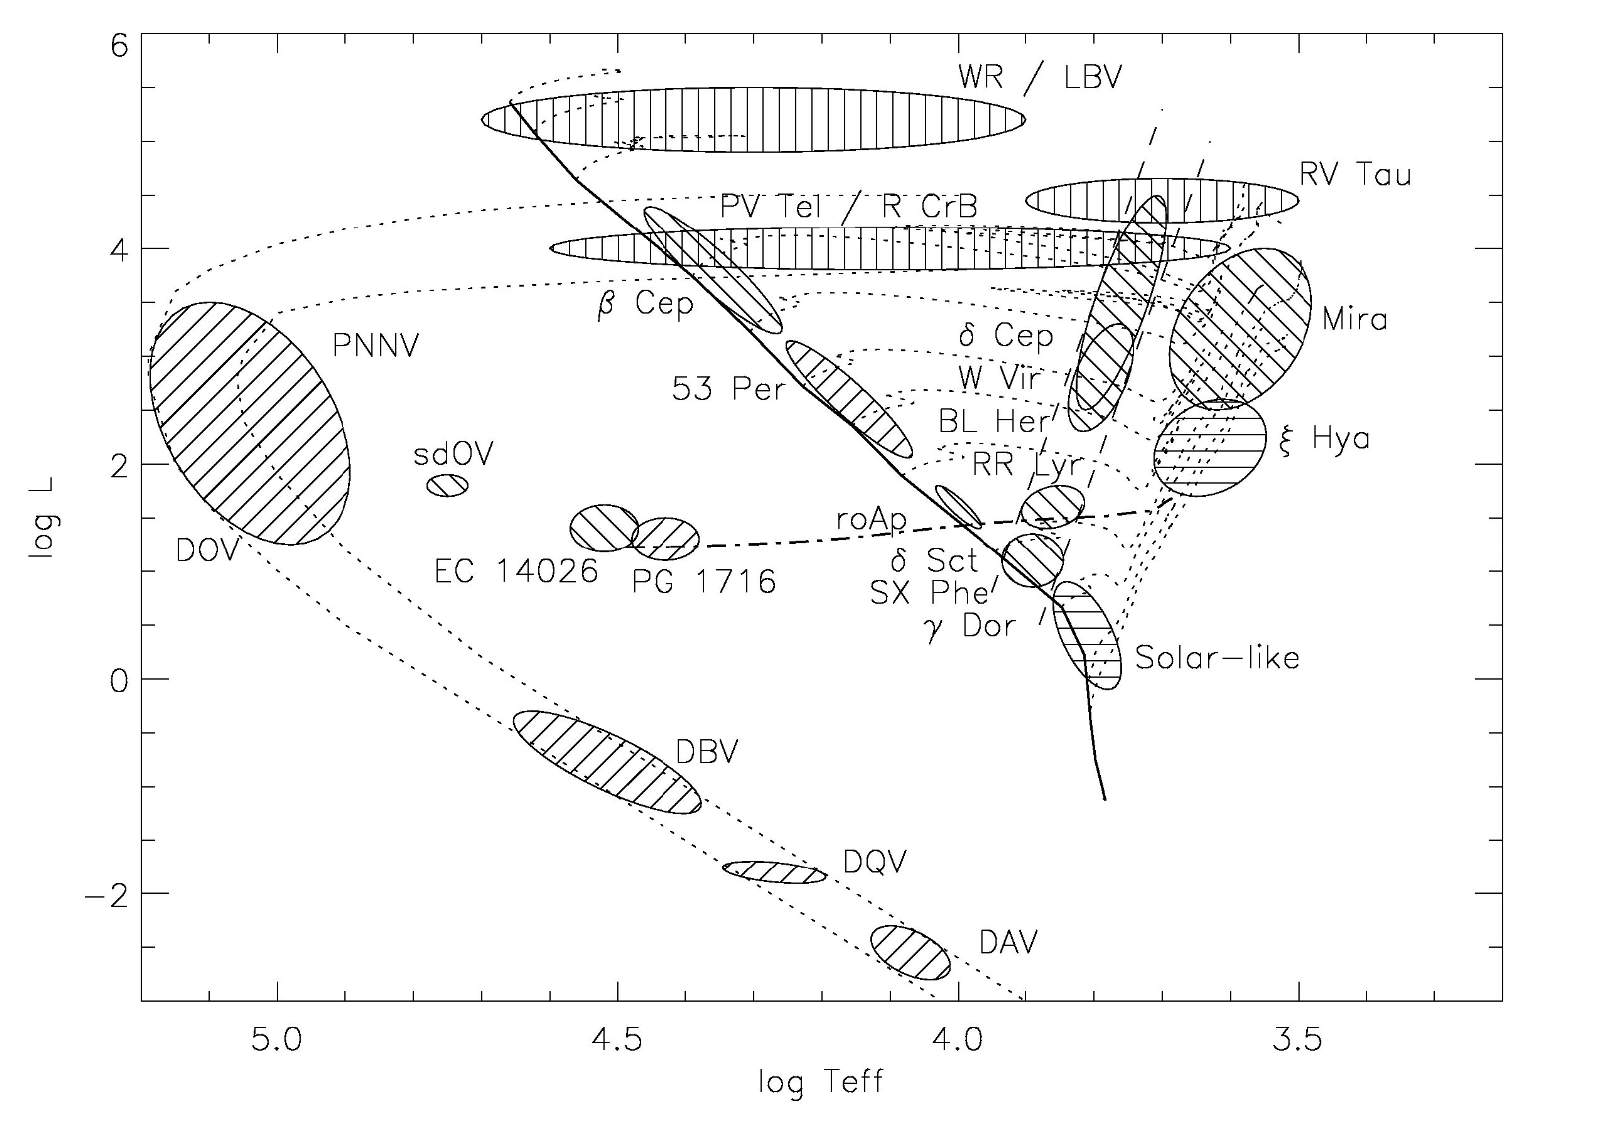
\includegraphics[width=\textwidth]{Imagenes/HR_Pulsating.png}
  \caption{Distribución de tipos de estrellas pulsantes en el diagrama HR. Figura tomada de \citet{2008CoAst.157..240J}.}
  \label{fig:hr_diagram_pulsating_stars}
\end{figure}

Existen diversas hipótesis para explicar la existencia de este tipo de estrellas. Por ejemplo: la transferencia de masa en sistemas binarios, las fusiones binarias, las colisiones estelares y la evolución atípica de estrellas individuales \citep{wang2024bluestragglerstars}. En este trabajo se busca diferenciar dos de ellas: la \textit{hipótesis aislada} y la \textit{hipótesis de transferencia de masa binaria}, mediante la astrosismología.

El modelo teórico de evolución estelar más simple asume una evolución aislada, es decir, que la estrella no interactúa con otros objetos celestes. En este caso, la explicación de la existencia de estas \textit{blue stragglers} es que son estrellas de una masa inicial alta, las cuales (por alguna razón desconocida) se formaron mucho más tarde que el resto de estrellas de su cúmulo. Esta es la \textit{hipótesis aislada}, y constituye nuestro modelo comparativo de control (\textit{baseline}).

La alternativa es que estas \textit{blue stragglers} se encuentren en sistemas binarios con otro objeto, el cual ha transferido parte de su material a la estrella (inicialmente con menor masa), provocando que esta se vuelva más masiva y caliente. Esta es la \textit{hipótesis de transferencia de masa binaria} \citep{wang2024bluestragglerstars}.

Estas dos hipótesis no pueden ser diferenciadas únicamente utilizando el diagrama HR. Dos estrellas con historias evolutivas completamente distintas pueden ubicarse en la misma posición, ocultando sus diferencias internas. Debido a ello se recurre a la astrosismología. Al estudiar las pulsaciones de dos estrellas en la misma posición pero con historias evolutivas distintas, se espera encontrar diferencias cuantificables en sus frecuencias de oscilación que permitan discernir cuál de las dos hipótesis es la correcta.

Esto lleva a la siguiente pregunta: ¿Qué tipo de observaciones astrosismológicas son necesarias para poder diferenciar entre estas dos hipótesis? Aquí es donde entra en juego la misión HAYDN.

\section{HAYDN}
La propuesta de misión HAYDN (acrónimo en inglés de High-precision AsteroseismologY in DeNse stellar fields) \citep{HAYDN} es una propuesta de misión espacial de clase media europea concebida en el marco del programa científico a largo plazo Voyage 2050 de la Agencia Espacial Europea. Actualmente, HAYDN se encuentra en fase de evaluación competitiva frente a otras propuestas para la misión M8 de la ESA, luego de haber superado la primera fase de selección y tener una buena base tras su evaluación inicial en la anterior convocatoria (M7). El proyecto está liderado por Andrea Miglio (Universidad de Bolonia) como Investigador Principal, y cuenta con un extenso consorcio internacional de más de 200 científicos (entre los que destaca Andrés Moya Bedón, tutor del presente proyecto, quien se desempeña como Investigador Principal de dicha misión en España y Co-Investigador Principal a nivel global.)

El objetivo de HAYDN es obtener series temporales fotométricas de alta precisión, alta cadencia y larga duración para grandes muestras de estrellas situadas en entornos estelares densos y ``controlados'', como son los cúmulos estelares abiertos (p. ej. $\chi$ y h Persei), cúmulos de edad intermedia (p. ej. M67), cúmulos globulares antiguos (p. ej. 47 Tuc y NGC 6397) y otras estructuras complejas, como son el bulbo de la Vía Láctea y Omega Centauri, hipotético remanente del cúmulo central de una galaxia absorbida por la Vía Láctea hace miles de millones de años \citep{Bekki_2003, haydn_mission_proposal_2026}.

En la década pasada, diversas misiones como CoRoT, Kepler y TESS han permitido obtener resultados con un alto valor científico en el marco de la astrosismología \citep{HAYDN,haydn_mission_proposal_2026, TASC8KASC15AbstractBooklet, IAUCommissionG4Report2024}. Sin embargo, el propósito de dichas misiones no era el estudio de las oscilaciones estelares, sino el de detectar exoplanetas a través del método de tránsitos en estrellas brillantes del campo galáctico. El problema que presentan para la toma de datos astrosismológicos en campos estelares densos es que emplean instrumentos con tamaños de píxel muy grandes en el cielo (TESS, por ejemplo, tiene píxeles que abarcan $20''$), y las \textit{Point-Spread-Functions} (PSFs) de las estrellas no son suficientemente pequeñas \citep{HAYDN,haydn_mission_proposal_2026}.

Esto impide tomar series fotométricas de estrellas individuales cuando estas se encuentran en campos altamente poblados, como son los cúmulos estelares densos y el centro galáctico debido a la severa contaminación por el solapamiento de la luz de estrellas vecinas. HAYDN soluciona esto empleando una escala del píxel del orden de $0.25''$ y un campo de visión más concentrado ($\lesssim 1^\circ$). Esto le permite resolver estrellas densamente agrupadas.

\begin{figure}[htpb]
  \centering
  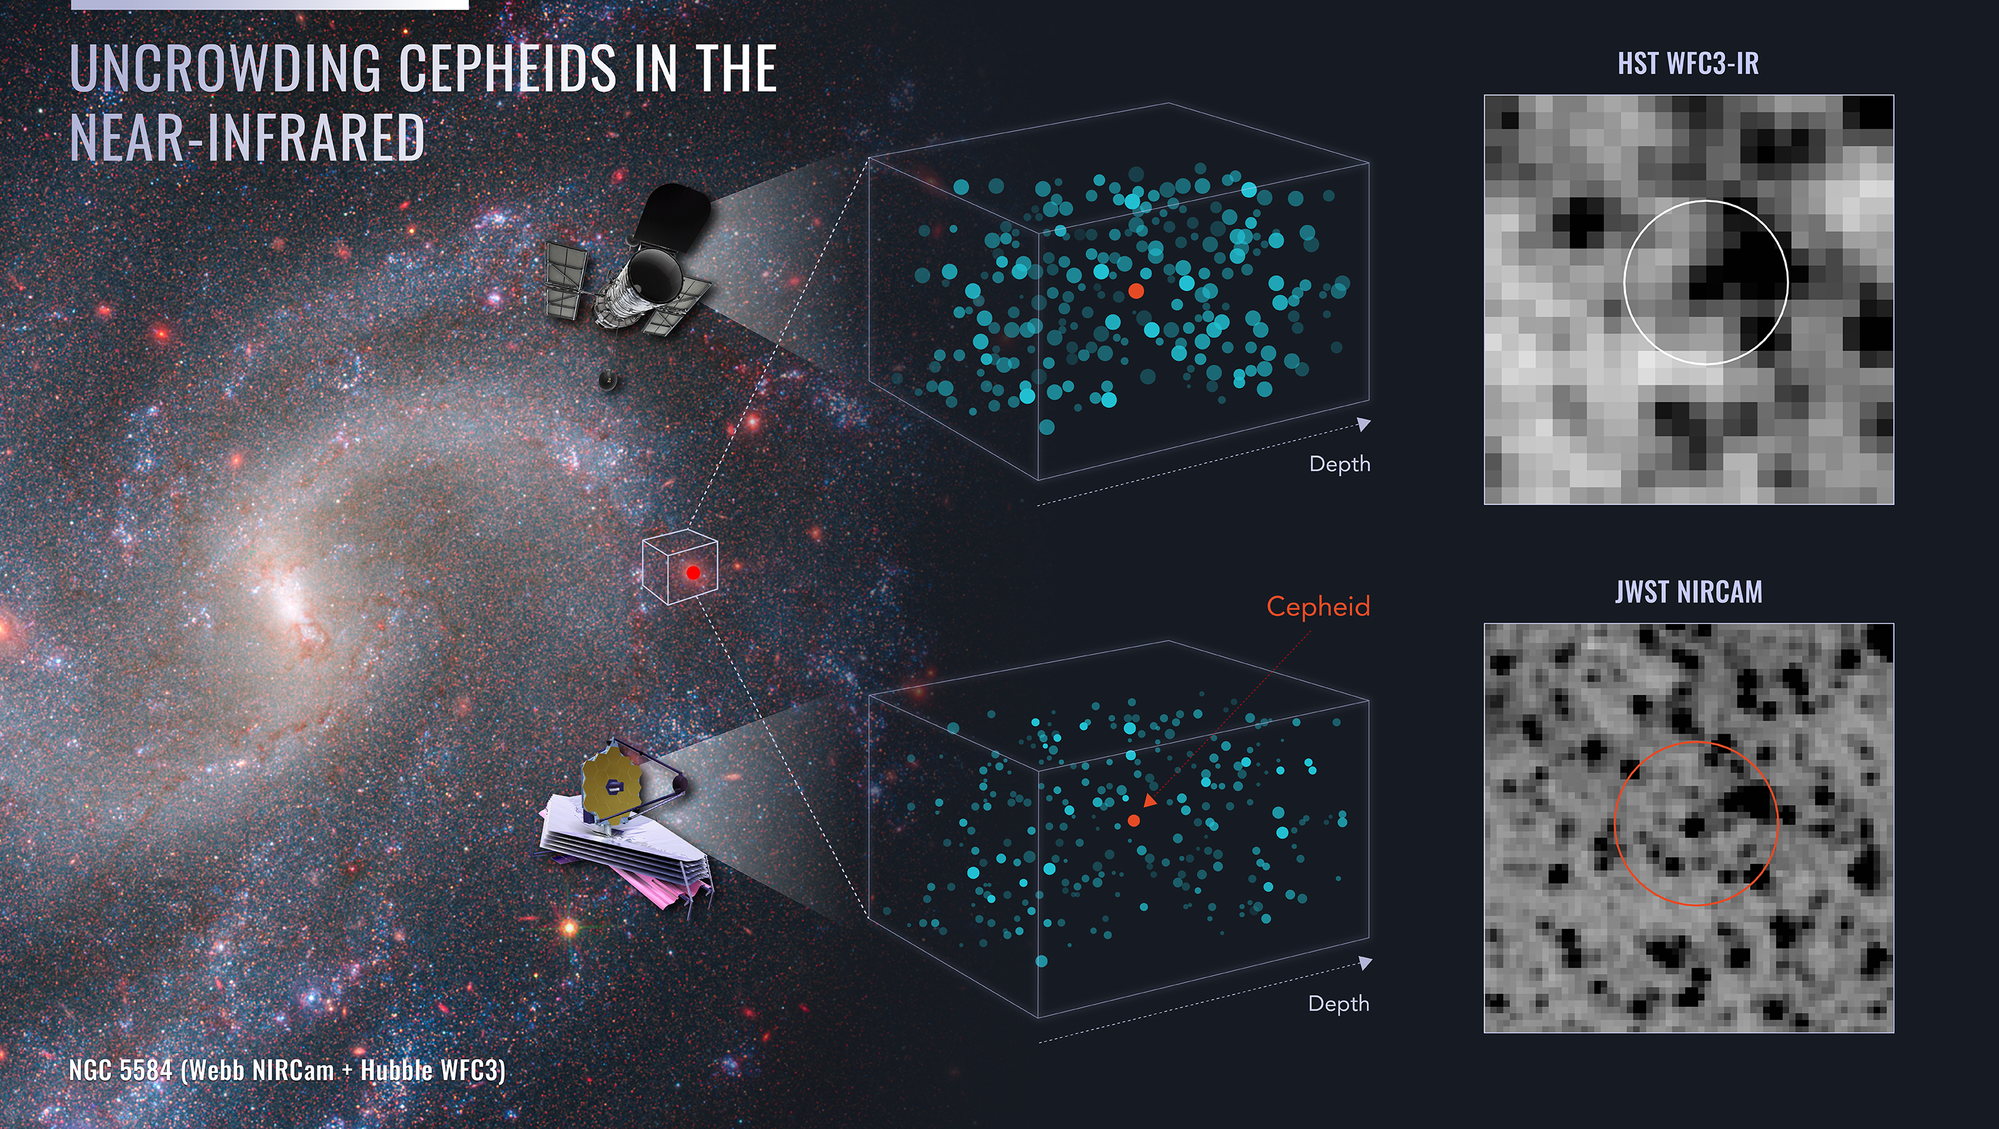
\includegraphics[width=0.8\textwidth]{Imagenes/cepheids.png}
  \caption{Imagen que muestra la galaxia NGC 5584. La visualización ilustra cómo el telescopio Webb (NIRCam) logra separar una estrella Cefeida (punto naranja) de la multitud de estrellas de fondo (puntos azules), una distinción que la menor resolución del Hubble (WFC3-IR) en el infrarrojo cercano no permitía hacer con claridad, como se ve en los recuadros ampliados. Imagen tomada de \citet{NASAWebb2023Cepheids}}
\end{figure}
\subsection{Objetivos y Arquitectura}

HAYDN proporcionará datos asterosísmicos sin precedentes en poblaciones estelares químicamente homogéneas y con edades bien determinadas. Esto le permitirá resolver preguntas clave en astrofísica. Para ello, se estructura en objetivos centrales que pueden agruparse de la siguiente manera \citep{HAYDN,haydn_mission_proposal_2026}:

\begin{itemize}
  \item \textbf{Astrofísica estelar y sistemas planetarios:} Se busca obtener restricciones sísmicas directas sobre procesos físicos internos, transporte de momento angular y pérdida de masa, enfocándose en estrellas masivas ($10$ -- $15~M_\odot$) progenitoras de objetos compactos. Además, investigará cómo el entorno de los cúmulos densos y diversos afecta la formación y características de los exoplanetas.
  \item \textbf{Calibración fundamental y arqueología galáctica:} Utilizará cúmulos estelares para refinar modelos físicos y calibrar escalas cósmicas de distancia y edad, lo que permitirá caracterizar el historial de formación de poblaciones estelares en entornos complejos (como el bulbo galáctico y galaxias enanas).
\end{itemize}

Estos objetivos se consiguen mediante una doble estrategia: una Muestra de Alta Precisión (HPS) para inferencia sísmica profunda y una Muestra de Sondeo (SS) para características poblacionales amplias. Los objetivos incluyen cúmulos de referencia (M67, 47 Tuc, $\chi$+ h Persei y el complejo $\omega$ Centauri), abarcando edades desde 10 Myr hasta 13 Gyr y metalicidades desde $\mathrm{[Fe/H]} \approx +0.1$ hasta $-2.0$ \citep{haydn_mission_proposal_2026}.

\subsection{Arquitectura y Operaciones}

Para cumplir sus objetivos, la misión HAYDN operará desde el punto de Lagrange L2 durante 4 años (con posibilidad de extensión), garantizando observaciones continuas sin fluctuaciones térmicas ni eclipses. Su arquitectura preliminar contempla:

\begin{itemize}
  \item Un espejo primario de 1.37 m de diámetro (equivalente a 120 cm sin obstrucción) con diseño óptico de dos espejos y tres reflexiones y un campo de visión de alrededor de $1^\circ$.

  \item Campañas de observación de larga duración (3, 6, 9 y hasta 18 meses continuos) sobre campos específicos, indispensables para obtener la resolución frecuencial necesaria para detectar la fina estructura de modos de pulsación mezclados y medir perfiles de rotación.

  \item Una importante colaboración con otros proyectos espectroscópicos terrestres e instrumentos, como el futuro HRMOS y los datos de la misión Gaia, lo que permitirá incrementar drásticamente su valor científico.
\end{itemize}

\vspace{1cm}
Antes de simular los modelos estelares y evaluar su posible detección observacional, es necesario establecer el marco físico y matemático que rige las pulsaciones en los interiores estelares.